\lecture{13}{11/11}

\begin{example}
    Let $f(x + iy) = xy + iy^2 = u(x, y) + iv(x, y)$ where $u(x, y) = xy$ and $v(x, y) = y^2$. Then
    \begin{align*}
        u_x &= y & u_y &= x \\
        v_x &= 0 & v_y &= 2y;
    \end{align*}
    hence, $f$ is only holomorphic at $(0, 0)$. Therefore $f$ is never complex differentiable on $\C^\star$ and so $f$ is not conformal at any point in $\C^\star$. We have
    \[ f'(0) = u_x(0,0) + iv_x(0,0) = 0; \]
    thus, $f$ is not conformal at $(0,0)$ either. 
\end{example}

\subsection*{Visualising conformal maps}

\begin{corollary}
    A \textbf{conformal map} maps orthogonal grids (of smooth curves) to orthogonal grides (of smooth curves).
\end{corollary}

\begin{example}
    Consider $f(z) = z^2 = (x^2 - y^2) + i(2xy)$ if $z = x + iy$. Consider the vertical line given by $x = a$, $a \in \R$, $a \neq 0$. Then \[ f(a + iy) = (a^2 - y^2) + i(2ay) = u + iv \]
    where $u = a^2 - y^2$ and $v = 2ay$. Thus
    \[ u = a^2 - \frac{v^2}{(2a)^2}. \]
    This is a parabola. The transformation of the line to the parabola is shown in Figure \ref{fig:conformal-map-ex-1} where $a = 1$. It is clear to see that the a similar sketch for the transformation of the line $z = x + i$ would show that the two parabolas intersect at right angles. 
\end{example}

\begin{figure}
    \centering
    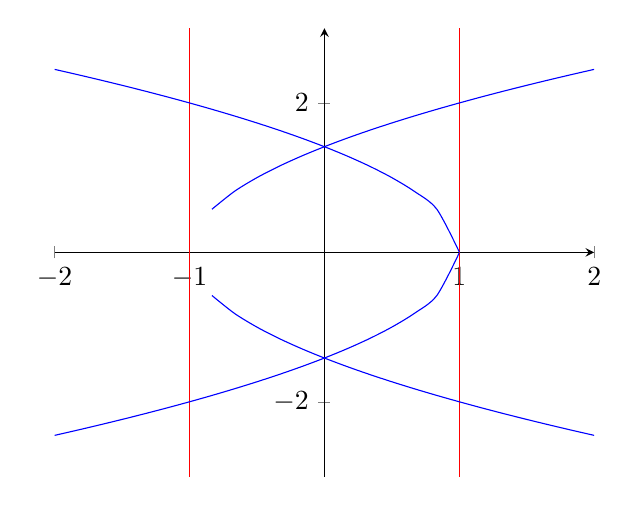
\begin{tikzpicture}
        \begin{axis}[axis lines=middle,
                     xmin=-2, xmax=2, ymin=-3, ymax=3]
            \addplot[red, smooth] coordinates {(1,-6) (1,6)};
            \addplot[red, smooth] coordinates {(-1,-6) (-1,6)};
            \addplot[blue, smooth, domain=-2:2] {(2 - 2*x)^0.5};
            \addplot[blue, smooth, domain=-2:2] {-(2 - 2*x)^0.5};
            \addplot[blue, smooth, domain=-2:2] {(2 + 2*x)^0.5};
            \addplot[blue, smooth, domain=-2:2] {-(2 + 2*x)^0.5};
        \end{axis}
    \end{tikzpicture}
    \caption{Argand diagram showing $z = 1 + iy$ (red) and $f(z) = z^2$ (blue).}
    \label{fig:conformal-map-ex-1}
\end{figure}

\begin{definition}[Biholomorphic]
    If $D_1, D_2$ are domains in $\C$ and if $f: D_1 \to D_2$ we say $f$ is a  \textbf{biholomorphism} (is \textbf{biholomorphic}) if
    \begin{enumerate}
        \item $f$ is holomorphic;
        \item $f$ is a bijection; and
        \item $f^{-1}: D_2 \to D_1$ is holomorphic.
    \end{enumerate}
    If such an $f$ exists, we say that $D_1$ is biholomorphic to $D_2$ and we denote it by $f: D_1 \xrightarrow{\sim} D_2$.
\end{definition}

\begin{example}
    \begin{enumerate}
        \item Consider $\exp: \C \to \C^\star$, we have that $\exp(z + 2\pi i) = \exp{z}$. 
            Hence, $\exp$ is not injective and so $\exp: \C \to \C*$ is not a biholomorphism. 
            However, we can find a domain that it is biholomorphic. 
            Let $D = \{ z \in \C : \Im(\C) \in (-\pi, \pi) \}$. 
            Then $\exp{D} = \C \setminus \R_{\leq 0}$ since if $z = x + iy$ then $e^z = e^x e^{iy}$ can get any non-zero modulus and any $\Arg{(e^z)} \in (-\pi, \pi)$ except $\pi$ itself. 
            We claim that 
            $\exp: D \to \C \setminus \R_{\leq 0}$ 
            is a biholomorphism. 
            The inverse if $\Log: \C \setminus \R_{\leq 0}$; hence, $\exp$ is a bijection on $D$. 
            $\Log$ is holomorphic, hence $\exp$ is biholomorphic.

        \item $f(z) = z^2$, where $f: \C \to \C$ is not injective as $f(1) = f(-1)$.
            Consider
            \[ \mathbb H_R = \{ z : \Re{(z)} > 0 \}. \]
            $f(\mathbb H_R) = \C \setminus\R_{\geq 0}$, 
            we can check that 
            $f: \mathbb H_R \to \C\setminus\R_{\geq 0}$ 
            by finding the inverse.
            $f^{-1} = \exp{\left(\frac12\log{x}\right)}$.
            This is a composition of holomorphic function and so is holomorphic; hence, $f$ is biholomorphic.
    \end{enumerate}
\end{example}

\begin{lemma}[Automorphism groups]
    Let $D \subset \C$ be a domain. The set of all biholomorphisms from $D$ to $D$, with multiplication given by composition is a \textbf{group} called the \textbf{automorphism group of $D$} denoted $\operatorname{Aut}{(D)}$.
\end{lemma}

\begin{proof}
    \begin{enumerate}
        \item Identity: given by $z \mapsto z$ on $D$ (obviously a biholomorphism).
        \item Inverse: if $f: D \to D$ is a biholomorphism, thus $f^{-1}$ is a biholomorphism.
        \item Associative: function composition is associative.
        \item If $f, g : D \to D$ are biholomorphic, then $f \circ g$ is holomorphic by the chain rule, but so is $(f \circ g)^{-1}$ is holomorphic and exists and so $f \circ g$ is biholomorphic.
    \end{enumerate}
\end{proof}
